\documentclass[12pt]{scrartcl}%{article} % Beginn der LaTeX-Datei

%Titel etc

\title{
\begin{flushright}
 
\includegraphics[scale=0.5]{HAW_Marke_RGB_300dpi.jpg}
\end{flushright}

\vspace{3cm}

IT-Systeme\\
Konzept
 
\vspace{3cm}

\LARGE Interaktive Videoinstallation mit\\
granularem Synthesizer
}
%\author{Dennis Jonca}
\date{30.  Oktober 2023} %hier können Sie ein Datum eingeben, auch leer, sonst wird es
         %automatisch erzeugt

% Kopf- und Fußzeilen

\usepackage[headsepline,%footsepline
]{scrlayer-scrpage}
\pagestyle{scrheadings}
\clearpairofpagestyles

\ihead{30.10.2023}
\chead{IT Systeme}
\ohead{Konzept}
\ifoot{}
\cfoot{}
\ofoot{\pagemark}

%% twocolumn

\usepackage{amsmath,amssymb}  % erleichtert Mathe 
\usepackage{enumerate}% schicke Nummerierung

\usepackage{graphicx} % für Grafik-Einbindung
%\usepackage{hyperref}

\usepackage[german]{babel}
\usepackage[T1]{fontenc}
\usepackage{lmodern}
\usepackage{textcomp}
 % Einstellungen, wenn man deutsch schreiben will, z.B. Trennregeln
\usepackage[utf8]{inputenc}  % für Unix-Systeme
  % ermöglicht die direkte Eingabe von Umlauten und ß
  % evt. obige Zeile ersetzen durch
  % \usepackage[ansinew]{inputenc}  % für Windows
  % \usepackage[applemac]{inputenc} % für den Mac


%%%%%%%%%%%%%%%%%%%%%%%%%%%%%%%%%%%%%%%%%%%%%%%%%%%%%%%%%%%%%%%%%%
%
%  ntheorem
%
\usepackage[thmmarks,amsmath,hyperref,noconfig]{ntheorem} 
  % erlaubt es, Sätze, Definitionen etc. einfach durchzunummerieren.
\newtheorem{satz}{Satz}[section] % Nummerierung nach Abschnitten
\newtheorem{hilfssatz}[satz]{Hilfssatz}
\newtheorem{kor}[satz]{Korollar}

\theorembodyfont{\upshape}
\newtheorem{beispiel}[satz]{Beispiel}
\newtheorem{bemerkung}[satz]{Bemerkung}
\newtheorem{definition}[satz]{Definition} %[section]

\theoremstyle{nonumberplain}
\theoremheaderfont{\itshape}
\theorembodyfont{\normalfont}
\theoremseparator{.}
\theoremsymbol{\ensuremath{_\blacksquare}}
\newtheorem{beweis}{Beweis}
\qedsymbol{\ensuremath{_\blacksquare}}
%\theoremclass{LaTeX}
%
% Ende ntheorem
%
%%%%%%%%%%%%%%%%%%%%%%%%%%%%%%%%%%%%%%%%%%%%%%%%%%%%%%%%%%%%%%%%%%


%\pagestyle{empty}
%
% Ändern der bedruckten Fläche der Seite
% \addtolength{\textwidth}{3cm}  % Befehl mit zwei Argumenten
% \addtolength{\textheight}{3cm}
% \hoffset-2cm % verschiebt das Textfenster nach links
% \voffset-5mm % verschiebt das Textfenster nach oben
%
%\parindent=0pt %% keine Einzug zu Beginn von Abs\"atzen
%\parskip=2mm   %% erzeugt einen zusätzliche Zeilenabstand zwischen
                %% Absätzen. Nötig bei \parindent=0pt


%%%%%%%%%%%%%%%%%%%%%%%%%%%%%%%%%%%%%%%%%%%%%%%%%%%%%%%%%%%%%%%%%%
% ermöglicht, farbigen Text zu drucken.
\usepackage{color}
% Und nun werden die Farben definiert - daran können Sie nach Belieben selber rumspielen.
\definecolor{white}{rgb}{1,1,1}
\definecolor{darkred}{rgb}{0.3,0,0}
\definecolor{darkgreen}{rgb}{0,0.3,0}
\definecolor{darkblue}{rgb}{0,0,0.3}
\definecolor{pink}{rgb}{0.78,0.09,0.51}
\definecolor{purple}{rgb}{0.28,0.24,0.55}
\definecolor{orange}{rgb}{1,0.6,0.0}
\definecolor{grey}{rgb}{0.4,0.4,0.4}
\definecolor{aquamarine}{rgb}{0.4,0.8,0.65}

\usepackage[table]{xcolor}% http://ctan.org/pkg/xcolor
\usepackage{lipsum}
\usepackage{wrapfig}



\DeclareMathOperator{\GL}{GL} % einige Macro, siehe am Ende Abschn. 2
\newcommand{\N}{\mathbb{N}}
\newcommand{\Z}{\mathbb{Z}}
\newcommand{\Q}{\mathbb{Q}}
\newcommand{\R}{\mathbb{R}}
\newcommand{\C}{\mathbb{C}}
\newcommand{\cP}{{\mathcal P}} 


\begin{document}

\begin{titlepage}


\maketitle % erzeugt den Kopf


\vfill 

\begin{flushleft}
\begin{tabular}{rlll}
%\cline{1-3}
\textbf{Gruppe:} & Ariane Bachmann (2xxxxxx) & Benjamin Ghodsi-Moghaddam (2xxxxxx) & \hspace{5cm} \\
 & Bruno Bühler (2xxxxxx) & Dennis Jonca (2xxxxxxx) & \hspace{5cm} \\
 & Fabian Brunner (2xxxxxx) & Rafael Weber (2xxxxxx) & \hspace{5cm} \\
& Tanggo Simamora (2xxxxxx) & & \hspace{5cm} \\\\
%\cline{1-3}
\textbf{Studiengang:} & Meidentechnik B.Sc. WS 23/24 & \hspace{5cm} \\\\
%\cline{1-3}
\textbf{eingereicht bei:} & Malte Sanders & \hspace{5cm} \\ 
%\cline{1-3}
\end{tabular}
\end{flushleft}



\end{titlepage}

\tableofcontents


\newpage

\section{Einleitung}

Im Rahmen des Kurses IT-Systeme soll ein interaktives Projekt entstehen, dass durch IT-Systeme realisiert ist. Dazu können die Studierenden Hard- und Software selbst auswählen und ihr eigenes Projekt entwickeln und umsetzen. Im Folgenden wird das Konzept des Projektes ''Visueller Synthesizer'' vorgestellt. 

\section{Product Vision}
\lipsum[2]
\section{Systembeschreibung}

Die Beschreibung des Systems soll helfen die Use-Cases und derer Umsetzung zu konkretisieren. Es werden die Anforderungen mithilfe der MoSCoW Methode aufgezeigt und die Bestandteile der Umsetzung durch ein Systemabbild dargestellt.

\subsection{MoSCoW Priorisierung}

Für das Projekt ist es am wichtigsten, dass die Produkt-Vision, demnach Audio und Video interaktiv zu gestalten, erfüllt wird. Viele weitere Funktionen sind dabei wünschenswert oder teilweise optional.
Es soll versucht werden, das Produkt möglichst verständlich für Menschen zu machen, die kein Verständnis für Synthesizern oder Videoanimation haben. Die Bedienung soll intuitiv und simpel sein.

\begin{enumerate}[]
\item \textbf{Must}
  \begin{enumerate}[-]
  \item Die Synthese der Audiospur wird verarbeitet.
  \item Audiospur wird interaktiv durch die Nutzenden verändert.
  \item Die Interaktion wird durch digitale Visualisierungen dargestellt.
  \end{enumerate}
\item \textbf{Should}
  \begin{enumerate}[-]
  \item Die Aufnahme am Mikrofon wird zur Verarbeitung gespeichert.
  \item granulare Synthese mit den Parametern Grain Pitch, Grain Speed, Grain Scan und Reverb.
  \item Visualisierungen werden durch TouchDesigner entwickelt und wiedergegeben.
  \end{enumerate}
\item \textbf{Could}
  \begin{enumerate}[-]
  \item Die Aufnahme am Mikrofon wird in Echtzeit verarbeitet.
  \item Die entstandene Waveform der Audiospur kann für die Nutzenden angezeigt werden.
  \item Der Audio-Pitch kann an einem MIDI-Keyboard gesteuert werden.
  \item Es gibt mehrere Designs durch TouchDesigner.
  \item Die Nutzenden können aus mehreren Designs selbst wählen.
  \end{enumerate}
\item \textbf{Won't}
  \begin{enumerate}[-]
  \item zu viele Ablenkungen des Users (zweite GUI, etc.)
  \item zu komplexe Bedienung des Controllers für die Nutzenden.
  \end{enumerate}
\end{enumerate}

\subsection{Der Systemaufbau}

Die Nutzenden haben mehrere Bedienungsmöglichkeiten. Ein Mikrofon, dessen Aufnahmen als Grundlage für den \emph{Granular Synthesizer} genutzt werden, Knöpfe zum starten und stoppen der Aufnahme des Mikrofons, Potentiometer und Slider, die die Steuerung der Synthesizer-Parameter ermöglichen. Außerdem ein MIDI-Keyboard für die Pitch-Kontrolle des Synthesizers
Es könnte auch eine Anzeige der Waveform geben, der von den Nutzdenden aufgenommenen Audiospur.\\\\
Der Mikrocontroller und das Keyboard senden MIDI-Daten an einen Computer in dem die Audiosynthese der zuvor aufgenommenen Audiodatei stattfindet.Das daraus resultierende Audiosignal wird einerseits über Lautsprecher in den Raum gespielt, und andererseits mit den MIDI-Daten zusammen an TouchDesigner weitergeleitet. Audio und MIDI haben Einfluss auf die Visualisierung, welche über HDMI durch einen Beamer in den Raum  wird.
\begin{center}
 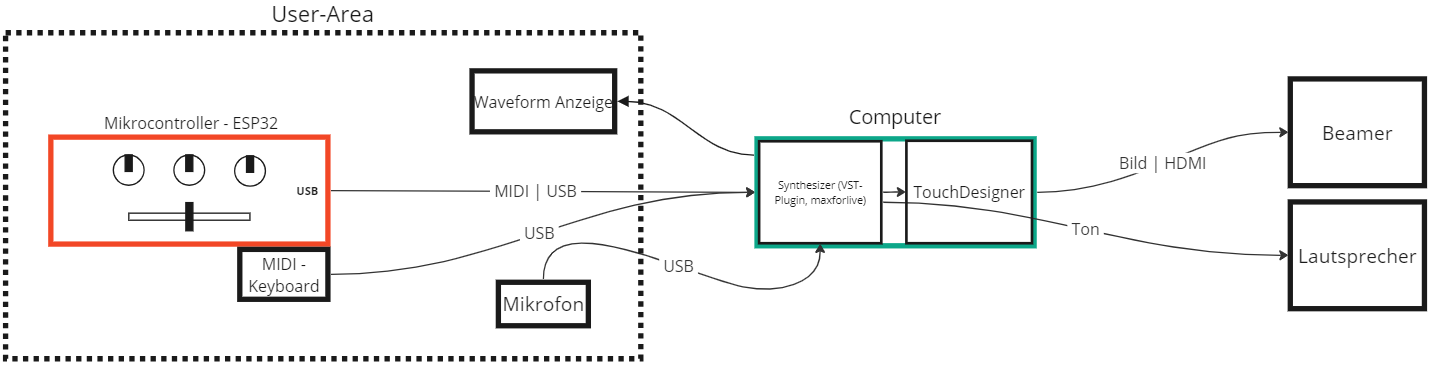
\includegraphics[scale=0.43]{system_schaltbild_v1.png}
 \captionof{figure}{Blockschaltbild des kompletten Systems}
\end{center}
\newpage
\subsection{Die Use Cases}
ddd
\begin{center}
 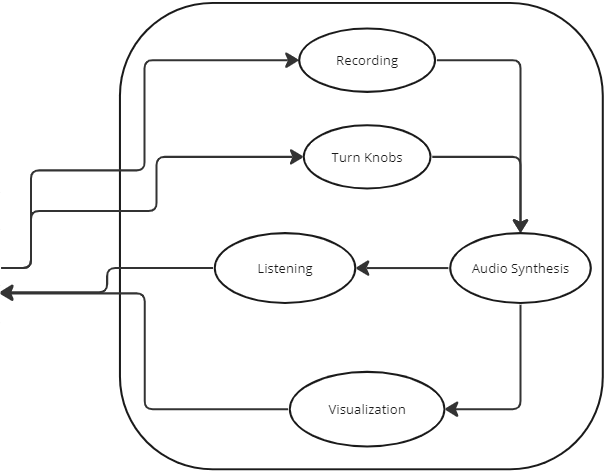
\includegraphics[scale=0.5]{usecases.png}
 \captionof{figure}{Usecase Diagramm des Projekts}
\end{center}
ddd
\section{Roadmap}

Die Roadmap soll einen zeitlichen Rahmen für das Projekt bieten. Es sind dort alle Projektwochen abgebildet und ein Ablaufplan ist konzipiert. Dieser kann sich während des Projektes gemäß des agilen Projektmanagements verändern.

\end{document}